% Data section. \input this from the main report file.
% Paths below assume the main .tex file sits in report/; change ../ if it doesn't.
% Numbers come from data/interim/data_stats.json. Figures and the filter table are
% rebuilt with `python -m src.data.figures`. Refers to \label{sec:methods}, which the
% Methods section should define.

\section{Data}
\label{sec:data}

\paragraph{Source.}
Our battles come from a public Hugging Face dataset of Pok\'emon Showdown
replays~\cite{holidayougi_replays,showdown}. It holds about 34 million replays
(73\,GB), 2.5 million of them in Gen~9 OU. Each replay is a text log of the whole
battle. We keep the 1{,}190{,}747 Gen~9 OU replays uploaded between June~1, 2025
and October~5, 2026, and from each log keep only three kinds of lines: the two
players with their ladder ratings, the six Pok\'emon each side shows at team
preview, and the winner. This shrinks the data from 6\,GB to 169\,MB. Each battle
becomes one example: two sets of six species, two ratings, and the label
$y = 1$ if player~1 won.

\paragraph{Cleaning and filtering.}
Table~\ref{tab:filters} lists every filter and how many battles it removes. Few
battles are broken (1.0\% do not list six Pok\'emon per side, 0.02\% have no
winner). Most of the drop is on purpose: we keep only battles where both players
are rated at least 1300, which removes the low ladder where new and casual
accounts play, and where the two ratings are within 100 points, so that the
teams, not a skill gap, decide most games. That leaves 533{,}490 clean battles,
from which we draw 100{,}000 uniformly at random (seed 42). The average rating in
the sample is 1510 and player~1 wins 49.8\% of the time, so neither side has a
built-in advantage.

\begin{table}[t]
  \centering
  \small
  % Written by `python -m src.data.figures` from data/interim/data_stats.json; don't edit.
\begin{tabular}{lrr}
\hline
Step & Battles left & Dropped \\
\hline
Gen 9 OU replays since 2025-06-01 & 1,190,747 & -- \\
log parses & 1,190,743 & 4 \\
exactly 6 Pok\'emon per side & 1,179,001 & 11,742 \\
has a winner (no tie) & 1,178,752 & 249 \\
both players rated & 1,147,643 & 31,109 \\
both ratings $\geq$ 1300 & 580,386 & 567,257 \\
rating gap $\leq$ 100 & 533,490 & 46,896 \\
\hline
random sample (seed 42) & 100,000 & \\
\hline
\end{tabular}

  \caption{Filters applied to the Gen~9 OU replays, in order. The rating filter
  removes the most battles by design.}
  \label{tab:filters}
\end{table}

\paragraph{Train, validation and test split.}
We split by upload time instead of at random (Figure~\ref{fig:split}): the oldest
70\% (70{,}000 battles, June~2025 to April~8, 2026) for training, the next 15\%
(to July~1, 2026) for validation, and the newest 15\% (to October~5, 2026) for the
test set. This matches real use, where a model trained on past battles predicts
future ones, and it keeps the test set honest: the popular teams and the
strongest picks drift over time, and a random split would let the model see the
test period during training. The cost is some shift between the splits; for
example the average rating is 1510 in train, 1483 in validation and 1534 in test.
Player~1 wins 49.8\%, 49.9\% and 49.7\% of the battles in the three splits.

\begin{figure}[t]
  \centering
  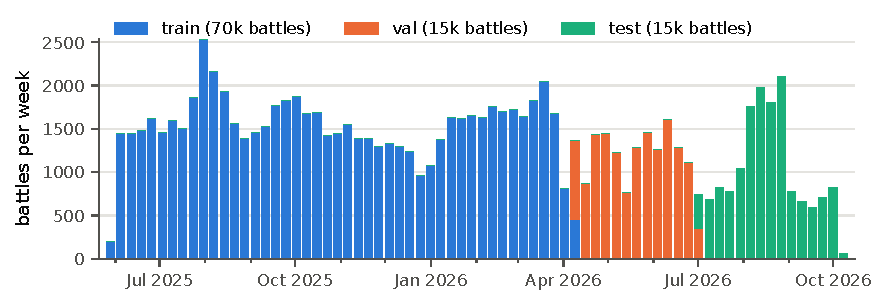
\includegraphics[width=\linewidth]{../figures/data_split_timeline.pdf}
  \caption{Battles per week in our 100{,}000-battle sample, colored by split. The
  split is by time, so validation and test are strictly newer than training.}
  \label{fig:split}
\end{figure}

\paragraph{Pok\'emon facts.}
To describe a team with numbers we also need each species' types, base stats and
possible abilities, and the type chart. We take these from Pok\'emon Showdown's
own data files through the poke-env library~\cite{showdown,pokeenv}. Cosmetic
forms that play identically (for example the colors of Alcremie) are merged into
their base species. Every species in our battles is in this Pok\'edex.

\paragraph{What the teams look like.}
After merging forms, 534 different species appear in the training battles, but
usage is very uneven (Figure~\ref{fig:species}): Great Tusk is on 31.5\% of
teams, and 402 species appear in at least 20 training battles, the cutoff we use
for giving a species its own feature. The win rates of the most common species
all lie between 49\% and 52\%. No single Pok\'emon wins games on its own, so any
signal has to come from combinations and matchups, which is what our features in
Section~\ref{sec:methods} try to capture. Because of the time split, a few
species are new in later months: 18 species that never appear in training show up
in 7.7\% of validation battles, and 13 in 2.0\% of test battles. They get no
species feature, only their types and stats.

\begin{figure}[t]
  \centering
  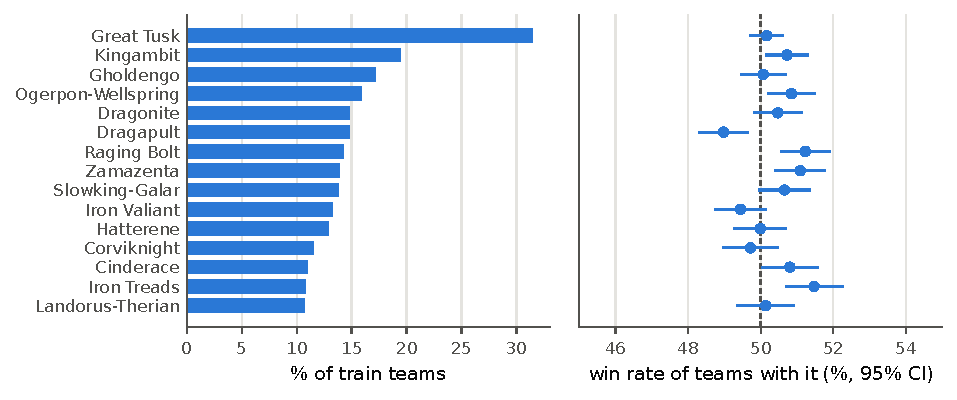
\includegraphics[width=\linewidth]{../figures/data_top_species.pdf}
  \caption{The 15 most used species in the training set. Left: share of teams
  that include the species. Right: win rate of those teams with a 95\% confidence
  interval; the dashed line marks 50\%.}
  \label{fig:species}
\end{figure}
